% Versi Bahasa Indonesia — dihasilkan oleh `paper-agent translate-tex` dari sections_id/ -> sections_id/
% Build: paper-agent compile paper/main_id.tex
\documentclass[conference]{IEEEtran}
\IEEEoverridecommandlockouts

\usepackage[utf8]{inputenc}
\usepackage[T1]{fontenc}
\usepackage[bahasa]{babel}
\usepackage{cite}
\usepackage{amsmath,amssymb,amsfonts}
\usepackage{graphicx}
\usepackage{booktabs}
\usepackage{array}
\usepackage{xcolor}
\usepackage{url}
\usepackage[hidelinks]{hyperref}
\usepackage{microtype}

\graphicspath{{figures/}}

\addto\captionsbahasa{%
  \def\abstractname{Abstrak}%
  \def\tablename{TABEL}%
  \def\refname{Daftar Pustaka}%
  \def\IEEEkeywordsname{Kata Kunci}%
}

% \todo{} marks items that must be resolved before submission
\newcommand{\todo}[1]{\textcolor{red}{[TODO: #1]}}
% placeholder token as it appears in the masked text, e.g. \ph{3}
\newcommand{\ph}[1]{\texttt{[[#1]]}}

\begin{document}

\title{Model Mana yang Sebenarnya Menjawab? Substitusi Model Senyap, Validator Deterministik, dan \emph{Routing} Multi-Model dalam Agen Paper Berbasis LLM}

\author{%
\IEEEauthorblockN{Andi Agung Dwi Arya B}
\IEEEauthorblockA{\textit{Program Studi Magister Teknik Informatika, Fakultas Teknik} \\
\textit{Universitas Hasanuddin}\\
Makassar, Indonesia \\
D082251054 $\cdot$ \todo{email}}
}

\maketitle

\begin{abstract}
Agen riset semakin sering memanggil large language models (LLMs) komersial melalui SDK vendor dan melaporkan nama model yang diminta sebagai provenans keluaran mereka. Kami menunjukkan bahwa label ini dapat salah: CLI penyedia menerima nama model apa pun dan, ketika akun tidak berhak mengaksesnya, secara diam-diam melayani model yang berbeda---Claude Opus 4.8 diminta dan Claude Haiku 4.5 menjawab, dan sebuah nama model fiktif juga ``succeeded''. Hanya event penggunaan penyedia yang menyebut nama model yang menjawab. Kami memasukkan pengamatan ini ke dalam \emph{paper-agent}, sebuah agen sumber terbuka untuk artikel ilmiah yang (i) merekam model yang melayani setiap panggilan, (ii) merutekan pekerjaan ke model berdasarkan peran, dan (iii) membungkus setiap keluaran model dengan validator deterministik. Terjemahan aman struktur menyamarkan LaTeX menjadi placeholder dan tag penekanan yang multiset dan pelekat-nomor-nya diverifikasi per unit. Pada sebuah makalah IEEE delapan bagian (146 unit, 4{,}673 kata, 262 placeholder) kami membandingkan sebuah pipeline tiga-model (draf, penyuntingan pasca oleh model yang berbeda, QA terjemahan balik oleh model lokal, seleksi per unit) dengan dua konfigurasi model tunggal. Pipeline dan model API tunggal sama-sama mempertahankan semua 146 unit tetap utuh secara struktural (model lokal kehilangan dua); kepatuhan glosarium pipeline (99.0\%) dan rata-rata cosine lintas bahasa (0.826 direct, 0.958 back-translation) \emph{tidak} lebih tinggi daripada model tunggal (99.7\%; 0.837, 0.961), dan memakan waktu dinding tiga kali lipat. Nilai tambahnya adalah penangkapan kesalahan: sebuah kalimat yang tersisa dalam bahasa Inggris, istilah teknis yang salah, dan placeholder yang dipindahkan di depan angka hanya ditemukan karena model kedua membaca ulang teks dan karena validator menolak keluaran yang cacat. Tiga kelas kesalahan---placeholder yang dipindahkan, model QA yang menggemakan inputnya, dan placeholder yang hilang---tidak terdeteksi oleh model manapun, termasuk penilai, melainkan oleh validator. Kami berargumen bahwa provenans model yang melayani dan validasi deterministik sebaiknya menjadi standar dalam agen riset, dan bahwa tinjauan multi-model terbaik diterapkan secara selektif.
\end{abstract}


\begin{IEEEkeywords}
model bahasa besar, routing model, provenans, terjemahan mesin, LaTeX, sistem AI komposit, LLM-sebagai-penilai, agen riset
\end{IEEEkeywords}

\section{Pendahuluan}
\label{sec:intro}

Perangkat lunak ilmiah yang dibangun di sekitar LLM kini secara rutin merupakan sistem \emph{komposit}: beberapa model, komponen retrieval dan pemeriksaan berbasis aturan bekerja sama, dan pemilihan model per langkah adalah variabel desain, bukan konstanta~\cite{chen2024compound,chen2023frugalgpt,ong2024routellm}. Agen riset yang membaca, menerjemahkan, meninjau atau meringkas makalah adalah kasus yang menonjol, dan hasil mereka masuk ke tesis dan publikasi bersama dengan pernyataan semacam ``the LLM was \texttt{model-X}''. Pernyataan itu merupakan bagian dari catatan ilmiah: ia menentukan apakah sebuah hasil dapat direproduksi dan apakah dua run dapat dibandingkan.

Paper ini dimulai dari sebuah insiden dalam sistem semacam itu. Sebuah agen neuro-simbolik untuk mendeteksi indikator synthesis gap dalam literatur ilmiah~\cite{arya2026wizard} memanggil model Claude melalui SDK komersial~\cite{copilotsdk2026} dan memberi label setiap hasil dengan model yang dikonfigurasi, Claude Opus 4.8 (identifier \texttt{claude-opus-4.8-fast}). Ketika hak akses akun berubah, CLI terus menerima nama tersebut---dan terus mengembalikan jawaban---sementara model lain, Claude Haiku 4.5, yang melakukan pekerjaan tersebut. Tidak ada apa pun dalam respons yang memberi sinyal substitusi; nama model fiktif diterima begitu saja. Satu-satunya bukti yang dapat diandalkan adalah sebuah event penggunaan (usage event) yang mencantumkan model yang menjawab. Label dalam tesis itu, selama suatu periode, salah.

Insiden ini menimbulkan pertanyaan umum bagi agen riset: \emph{model mana yang sebenarnya menjawab, dan bagaimana agen sebaiknya mengetahui, mencatat, dan memanfaatkan hal itu?} Kami mengubah pertanyaan tersebut menjadi tiga pertanyaan penelitian.
\begin{itemize}
  \item \textbf{RQ1} Apakah model yang menjawab suatu permintaan sama dengan model yang diminta, dan mekanisme apa yang memberikan agen sebuah label provenans yang benar?
  \item \textbf{RQ2} Pada tugas yang sensitif terhadap struktur---menerjemahkan sebuah paper LaTeX sambil menjaga kutipan, matematika, dan silang-referensi tetap utuh---apakah sebuah pipeline yang menggabungkan beberapa model (penerjemah, penyunting, penilai) mengungguli satu model tunggal, dan dengan biaya apa?
  \item \textbf{RQ3} Kesalahan mana yang tertangkap oleh model (model kedua yang membaca ulang keluaran) dan mana yang hanya tertangkap oleh validator deterministik?
\end{itemize}

Kami menjawabnya dengan \emph{agen paper}, sebuah agen sumber terbuka untuk paper ilmiah yang setiap panggilan LLM-nya mencatat model yang menjawab, merutekan pekerjaan ke model berdasarkan peran, dan memvalidasi setiap keluaran model secara deterministik. Kontribusinya adalah:
\begin{itemize}
  \item sebuah laporan empiris tentang substitusi model senyap dalam SDK vendor dan sebuah mekanisme provenans (pencatatan model yang melayani, peringatan substitusi, label provenans yang benar) yang kami rekomendasikan untuk agen riset;
  \item sebuah metode terjemahan yang aman struktur untuk LaTeX yang menyamarkan perintah, matematika, dan referensi menjadi placeholder serta menempatkan penekanan ke dalam tag, memverifikasi multiset mereka dan keterikatannya pada angka per unit, dan mereproduksi sumber byte demi byte ketika tidak ada terjemahan yang diterapkan;
  \item perbandingan terkontrol antara sebuah pipeline tiga-model dengan dua konfigurasi model tunggal pada 146 unit yang sama, dengan metrik per-unit (cosine lintas bahasa, cosine terjemahan balik, kepatuhan glosarium, integritas struktur, waktu, model yang melayani) yang dirilis bersama kode;
  \item sebuah analisis kesalahan yang menunjukkan bahwa manfaat pipeline terletak pada menangkap kesalahan daripada meningkatkan rata-rata, dan bahwa tiga kelas kesalahan tidak terlihat oleh setiap model, termasuk penilai, namun tertangkap oleh validator.
\end{itemize}
Agen tersebut juga memverifikasi referensi terhadap basis data bibliografis, mengatur gerbang sitasi, membangun dan memeriksa PDF, meninjau sebuah paper dengan dua kritikus independen, dan mengonversi manuskrip Word ke IEEE LaTeX; fungsi-fungsi ini dijelaskan sebagai bagian dari sistem tetapi dievaluasi hanya secara informal di sini. Versi bahasa Indonesia dari paper ini diproduksi oleh agen itu sendiri.

\section{Pekerjaan Terkait}
\label{sec:related}

\paragraph{Sistem komposit, routing (perutean) dan ensembel}
FrugalGPT menunjukkan bahwa mengkaskadiakan model murah dan mahal dapat menyamai model kuat dengan sebagian kecil biaya~\cite{chen2023frugalgpt}; RouteLLM mempelajari router dari data preferensi~\cite{ong2024routellm}; LLM-Blender memberi peringkat dan memadukan keluaran beberapa model~\cite{jiang2023blender}; Mixture-of-Agents melapiskan model yang saling menyempurnakan jawaban satu sama lain~\cite{wang2024moa}. Chen et al.\  mengamati bahwa lebih banyak pemanggilan tidak membantu secara monoton dan bahwa manfaatnya bergantung pada distribusi kesulitan tugas~\cite{chen2024compound}. Pipeline kami adalah sistem komposit kecil dengan peran tetap; kontribusi kami bukan router yang lebih baik melainkan temuan bahwa nilai kombinasi pada tugas kami muncul dalam penangkapan kesalahan daripada dalam kualitas rata-rata, dan bahwa validator deterministik adalah komponen yang paling banyak menangkap.

\paragraph{Model menilai model}
LLM-sebagai-penilai setuju dengan manusia pada tingkat kesepakatan antar-anotator pada tugas chat~\cite{zheng2023judge}, dan umpan balik diri secara iteratif meningkatkan banyak tugas generasi~\cite{madaan2023selfrefine,shinn2023reflexion}. Dua temuan memperingatkan terhadap penggunaan satu model tunggal untuk menilai dirinya sendiri: LLM tidak dapat secara andal mengoreksi penalaran sendiri tanpa sinyal eksternal~\cite{huang2024selfcorrect}, dan evaluator LLM mengenali serta lebih menyukai generasi mereka sendiri~\cite{panickssery2024selfpref}. Oleh karena itu kami menggunakan model \emph{yang berbeda} sebagai penyunting, model ketiga untuk terjemahan balik, dan tidak pernah membiarkan sebuah model menjadi penentu tunggal validitas struktural.

\paragraph{Estimasi kualitas terjemahan mesin}
Metrik berbasis referensi seperti COMET~\cite{rei2020comet} memerlukan referensi manusia yang tidak kami miliki; annotasi MQM oleh pakar~\cite{freitag2021mqm} adalah standar emas tetapi mahal. Terjemahan bolak-balik telah ditinjau kembali sebagai estimator bebas referensi~\cite{moon2020roundtrip}, model kelas GPT kompetitif sebagai penerjemah~\cite{hendy2023gpt} dan merupakan evaluator terjemahan terdepan~\cite{kocmi2023gemba}. Kami menggabungkan kesamaan embedding kalimat lintas bahasa~\cite{reimers2019sbert,reimers2020multilingual} dengan terjemahan balik oleh model lokal~\cite{gemma2025}; terjemahan balik sebagai teknik berakar dari augmentasi data~\cite{sennrich2016backtranslation}. Konsistensi terminologi, yang ditegakkan dalam penerjemahan mesin neural melalui dekoding terkendali~\cite{dinu2019terminology}, ditangani di sini oleh glosarium dalam prompt dan diukur secara deterministik setelahnya.

\paragraph{Provenans dan dokumentasi model}
Model cards~\cite{mitchell2019modelcards} mendokumentasikan apa itu sebuah model; survei halusinasi~\cite{ji2023hallucination} mendokumentasikan apa yang mungkin dibuat-buat olehnya. Keduanya mengandaikan bahwa sistem mengetahui model mana yang sedang digunakannya. Dokumentasi vendor mencantumkan model mana yang dapat digunakan setiap paket langganan~\cite{githubdocs2026models} dan papan peringkat independen mengurutkannya untuk tugas ala riset~\cite{artificialanalysis2026}, tetapi keduanya tidak memberitahu agen yang berjalan model apa yang disajikan kepadanya. Agen bergaya ReAct~\cite{yao2023react} yang bertindak atas hasil alat akan sama-sama bertindak berdasarkan label model yang salah; kami menambahkan model yang melayani ke jejak.

\section{Desain Sistem}
\label{sec:method}

\begin{figure*}[t]
  \centering
  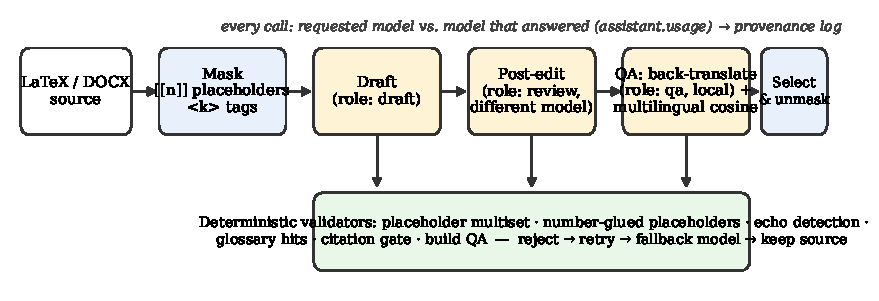
\includegraphics[width=0.92\textwidth]{fig1_architecture.pdf}
  \caption{Terjemahan aman struktur dalam agen paper. LaTeX disamarkan menjadi placeholder dan tag; tiga peran model (pembuatan draf, penyuntingan pasca, QA) diisi oleh model yang berbeda; validator deterministik berada di bawah setiap panggilan model dan menolak keluaran yang cacat (mencoba ulang, model cadangan (fallback), akhirnya mempertahankan sumber). Setiap panggilan mencatat model yang diminta dan model yang melayani.}
  \label{fig:arch}
\end{figure*}

Gambar~\ref{fig:arch} menunjukkan jalur terjemahan agen paper; perintah lain (verifikasi referensi, gerbang sitasi, membangun QA, tinjauan dua kritikus, konversi DOCX, perencanaan tugas berbahasa alami) menggunakan mesin, peran, dan log provenans yang sama. Agen tersebut adalah paket Python dengan antarmuka baris perintah dan API HTTP; setiap panggilan LLM melewati salah satu dari dua mesin, server Ollama lokal atau SDK GitHub Copilot~\cite{copilotsdk2026}.

\subsection{Provenans model yang melayani}
\label{sec:prov}
SDK Copilot menjalankan CLI vendor sebagai subproses dan menyediakan API sesi. Kami mengamati bahwa sesi yang dibuat dengan sembarang string \texttt{model} menjawab; ketika akun tidak berhak atas model, model lain digunakan dan tidak ada kesalahan atau bidang dalam respons yang menunjukkan hal itu. Namun, sesi tersebut memancarkan event \texttt{assistant.usage} yang bidang \texttt{model}-nya menyebut model yang menghasilkan token. Mesin berlangganan ke event ini untuk setiap panggilan, mengembalikan teks bersama dengan model yang melayani, menghitung model yang diminta dan model yang melayani secara terpisah, dan mencetak peringatan satu kali untuk setiap pasangan (model yang diminta, model yang melayani). Semua laporan yang dihasilkan oleh agen (laporan terjemahan, laporan tinjauan, ringkasan run tugas) memuat model yang melayani. Mesin lokal mencatat nama model yang dikembalikan oleh server, yang selalu merupakan model yang diminta.

\subsection{Peran model}
Pekerjaan dialokasikan kepada \emph{peran}, bukan kepada model: \textsc{draft} (penerjemah), \textsc{review} (penyunting), \textsc{qa} (penerjemah balik), \textsc{fallback}, \textsc{critic} dan \textsc{critic2} (peninjau independen), \textsc{planner}. Pengikatan default mencerminkan model-model yang dapat diakses oleh langganan Copilot paket dasar---\texttt{gpt-5-mini} untuk pembuatan draf, \texttt{claude-haiku-4.5} untuk penyuntingan pasca dan kritik---ditambah \texttt{gemma3:27b}~\cite{gemma2025} lokal untuk QA, cadangan (fallback) dan kritikus kedua; pengikatan ini digantikan oleh variabel lingkungan. Dua aturan tetap: penyunting tidak pernah menjadi model pembuat draf, dan kedua kritikus tidak pernah merupakan model yang sama~\cite{panickssery2024selfpref,huang2024selfcorrect}.

\subsection{Penyamaran aman struktur}
\label{sec:mask}
Setiap baris dari file bagian LaTeX dibagi menjadi \emph{unit} yang dapat diterjemahkan: sebuah paragraf, argumen dari \verb|\section|/\verb|\caption|/\verb|\paragraph|, sebuah sel tabel (baris dipisah pada top-level \verb|&|), atau sebuah \verb|\item| body. Baris yang murni struktur (\verb|\begin|, \verb|\label|, \verb|\includegraphics|, rules, comments) dipertahankan verbatim. Di dalam sebuah unit, matematika (\verb|$...$|), sitasi, referensi, label, identifier (\verb|\texttt|, \verb|\textsc|), grup kurung kurawal, \verb|~|, \verb|\%| dan setiap perintah lain beserta argumennya diganti oleh placeholder bernomor \ph{n}; rentang yang dimaskir bersebelahan digabung menjadi satu placeholder. Perintah penekanan \verb|\emph|, \verb|\textbf| dan \verb|\textit| menjadi tag inline \verb|<k>...</k>| yang isinya tetap diterjemahkan. Pembukaan samaran membalik kedua operasi tersebut, meng-escape bare specials yang mungkin diketik model (\verb|%|, \verb|"&|, \verb|\_|), menormalkan tanda kutip tipografi dan tanda hubung kembali ke LaTeX, serta mengembalikan spasi awal dan akhir unit. Penyamanaran yang diikuti pembukaan samaran tanpa penerjemahan mereproduksi setiap byte file sumber byte demi byte; ini adalah uji unit dan pemeriksaan dry-run terhadap alat. Satu lintasan deterministik akhir menulis ulang kata sebelum \verb|~\ref| (``Fig.'', ``Table'', ``Section'') ke dalam bahasa tujuan, karena model kadang-kadang membiarkannya tidak diterjemahkan.

\subsection{Validator Deterministik}
\label{sec:validators}
Setiap keluaran model untuk sebuah unit hanya diterima jika (i) multiset placeholder sama dengan multiset sumber, (ii) multiset tag sama dengan multiset sumber, dan (iii) setiap placeholder yang menempel pada angka dalam sumber (``58\ph{3}'' yang berarti \verb|58\%|) menempel pada angka yang sama dalam keluaran (koma desimal ditoleransi). Keluaran yang ditolak dicoba ulang, kemudian dikirim ke model cadangan (fallback), dan akhirnya teks sumber dipertahankan serta unit dilaporkan sebagai tidak diterjemahkan. Terjemahan balik yang sama dengan inputnya ditolak sebagai panggilan QA yang gagal. Setelah run, kepatuhan glosarium diukur sebagai proporsi istilah sumber glosarium yang ada dalam sebuah unit yang istilah targetnya muncul dalam keluaran. Semangat yang sama mengatur perintah lain: sebuah gerbang sitasi menolak setiap kunci \verb|\cite| yang tidak ada di bibliografi atau tidak terverifikasi dalam setidaknya dua sumber bibliografis, dan langkah build melaporkan halaman, referensi yang tidak terdefinisi dan penanda TODO yang tersisa.

\subsection{Pipeline dan seleksi}
\label{sec:pipelines}
Pipeline \textsc{multi} menjalankan \textsc{draft}, lalu \textsc{review} dengan sumber dan draf (penyunting mengembalikan teks yang disempurnakan dan catatan satu baris tentang apa yang diubah), lalu \textsc{qa}: kedua kandidat diterjemahkan balik ke bahasa Inggris oleh model lokal dan dinilai oleh $q=\tfrac12(\cos(s,t)+\cos(s,b))$, di mana $s$ adalah sumber yang disamarkan, $t$ kandidat dan $b$ terjemahan baliknya, menggunakan model embedding kalimat multibahasa \texttt{paraphrase-multilingual-MiniLM-L12-v2}~\cite{reimers2020multilingual} dengan placeholder dan tag dihapus. Versi yang ditinjau dipilih kecuali skornya lebih dari $0.02$ di bawah skor draf. Pipeline \textsc{single} menggunakan satu model untuk pembuatan draf dan tanpa penyuntingan pasca; QA tetap dihitung sehingga konfigurasi dapat dibandingkan. Unit dikirim dalam batch sekitar 2{,}500 karakter sebagai JSON; dua batch dijalankan secara bersamaan.

\subsection{Perintah Lain}
\emph{verify-refs} mencocokkan setiap entri dari seed yang dikurasi (judul, penulis, tahun, DOI opsional atau id arXiv) terhadap Crossref, OpenAlex, Semantic Scholar, Scopus dan arXiv; suatu entri dianggap \textsc{verified} ketika kesamaan judul $\ge0.90$ dan tahun $\pm1$ terpenuhi pada setidaknya dua sumber, DOI seed yang salah dilaporkan dan diganti, serta BibTeX diambil dari doi.org dan divalidasi terhadap seed. \emph{review} mengirim paper yang dipipihkan ke dua kritikus dengan rubrik tetap dan menggabungkan temuan mereka, menandai isu yang diangkat oleh keduanya; setiap temuan menyertakan model yang melayani. \emph{docx2tex} mengonversi manuskrip Word menjadi proyek IEEEtran (heading, runs, tabel, gambar, kutipan numerik, daftar referensi sebagai seed yang belum terverifikasi). \emph{run} mengubah permintaan berbahasa alami menjadi rencana atas alat-alat ini, yang dibuat oleh model perencana atau oleh router kata kunci, dengan semua jalur dibatasi pada direktori kerja.

\section{Pengaturan Eksperimental}
\label{sec:setup}

\paragraph{Eksperimen A: substitusi (RQ1)}
Melalui Copilot SDK, dengan token akses personal yang terperinci dari akun paket dasar, kami meminta model yang akun tersebut berhak gunakan (\texttt{claude-haiku-4.5}, \texttt{gpt-5-mini}), sebuah model yang tidak berhak digunakannya (\texttt{claude-opus-4.8-fast}) dan sebuah nama fiktif, serta membaca model yang melayani dari event penggunaan (Bagian~\ref{sec:prov}). Perilaku tersebut ditunjukkan oleh uji otomatis pada agen yang awalnya mengalami insiden~\cite{arya2026wizard}.

\paragraph{Eksperimen B: konfigurasi terjemahan (RQ2)}
Materi adalah paper konferensi IEEE pendamping~\cite{arya2026wizard}: delapan berkas bagian, 146 unit, 4{,}673 kata, 262 placeholder dan 38 tag penekanan setelah penyamaran; 51 unit adalah sel tabel, 44 adalah judul bagian atau keterangan, 7 adalah butir daftar dan 44 adalah paragraf. Sasaran adalah Bahasa Indonesia formal dengan glosarium 103 istilah yang diturunkan dari tesis yang dirangkum oleh paper (mis.\ \emph{synthesis gap}, \emph{rule engine} dan \emph{knowledge graph} tetap dalam Bahasa Inggris; \emph{fragmentation} $\rightarrow$ \emph{fragmentasi}). Tiga konfigurasi menerjemahkan unit yang sama dengan glosarium dan prompt yang sama (Tabel~\ref{tab:configs}). Setiap konfigurasi dijalankan sekali; model API dijalankan dengan sampling default vendor, model lokal pada temperature $0.2$. Perangkat keras: dua NVIDIA L40S (46~GB) untuk Ollama; \texttt{gemma3:27b} dalam kuantisasi 4-bit.

\begin{table}[t]
  \caption{Konfigurasi yang dibandingkan dalam Eksperimen B. QA (terjemahan balik + cosine) dihitung untuk ketiganya.}
  \label{tab:configs}
  \centering
  \footnotesize
  \setlength{\tabcolsep}{3pt}
  \begin{tabular}{@{}lp{1.75cm}p{1.95cm}p{1.6cm}@{}}
    \toprule
    Konfigurasi & Draf & Sunting pasca & Seleksi \\
    \midrule
    \textsc{multi} & GPT-5 mini (Copilot) & Claude Haiku 4.5 (Copilot) & per unit berdasarkan skor QA \\
    \textsc{single}-Haiku & Claude Haiku 4.5 (Copilot) & -- & -- \\
    \textsc{single}-gemma3 & Gemma 3 27B (local, 4-bit) & -- & -- \\
    \bottomrule
  \end{tabular}
\end{table}

\paragraph{Metrik}
(i) integritas struktur: unit yang outputnya lolos validator (Bagian~\ref{sec:validators}) dan unit yang dibiarkan dalam bahasa Inggris; (ii) kepatuhan glosarium; (iii) rata-rata cosine lintas bahasa antara teks sumber dan teks akhir serta antara sumber dan terjemahan balik dari teks akhir; (iv) untuk \textsc{multi}, rasio suntingan penyunting pasca ($1-$ kesamaan difflib antara draf dan teks yang ditinjau) dan hasil seleksi; (v) waktu dinding, detik-model per unit, jumlah panggilan API dan model yang melayani; (vi) kesepakatan antar konfigurasi sebagai kesamaan tingkat karakter rata-rata dari teks akhir mereka. Nilai cosine dihitung dengan model embedding yang sama untuk semua konfigurasi dan dilaporkan beserta galat bakunya.

\paragraph{Eksperimen C: analisis kesalahan (RQ3)}
Kami memeriksa setiap unit yang validatornya terpicu, setiap unit yang skor QA-nya turun lebih dari $0.10$ setelah penyuntingan pasca, catatan perubahan penyunting pasca, dan unit bernilai terendah dari setiap konfigurasi, dan mengklasifikasikan apa yang menangkap setiap kesalahan: model penyuntingan pasca, model QA, atau validator.

\section{Hasil}
\label{sec:results}

\subsection{Eksperimen A: Model yang melayani bukan model yang diminta}
Tabel~\ref{tab:served} merangkum uji substitusi. Model yang berhak dilayani sesuai dengan permintaan. Setiap nama yang tidak berhak---termasuk yang fiktif---diterima tanpa kesalahan dan dijawab oleh Claude Haiku 4.5. Tidak ada bidang dari objek respons yang berbeda antara kedua kasus; hanya event penggunaan (usage event) yang menamai model yang melayani. Agen yang menampung insiden tersebut telah memberi label beberapa bulan analisis dengan nama yang diminta; label-labelnya sekarang diturunkan dari event penggunaan (usage event), sebuah peringatan substitusi dicatat sekali per pasangan, dan endpoint kesehatan-nya melaporkan autentikasi secara eksplisit, karena login yang kadaluarsa sebelumnya hanya muncul sebagai hasil kosong.

\begin{table}[t]
  \caption{Eksperimen A: model yang diminta versus model yang melayani melalui SDK vendor pada akun paket dasar (berhak: Claude Haiku 4.5, GPT-5 mini, GPT-5.3 Codex, GPT-4.1). Tidak ada permintaan yang menghasilkan kesalahan.}
  \label{tab:served}
  \centering
  \footnotesize
  \begin{tabular}{@{}ll@{}}
    \toprule
    Diminta & Dilayani (event penggunaan (usage event)) \\
    \midrule
    Claude Haiku 4.5 & Claude Haiku 4.5 \\
    GPT-5 mini & GPT-5 mini \\
    Claude Opus 4.8 & Claude Haiku 4.5 \\
    nama fiktif & Claude Haiku 4.5 \\
    \bottomrule
  \end{tabular}
\end{table}

\subsection{Eksperimen B: Tiga Konfigurasi, Unit yang Sama}
Tabel~\ref{tab:results} dan Gambar~\ref{fig:configs} melaporkan perbandingan tersebut. Ketiga konfigurasi menghasilkan paper bahasa Indonesia yang dapat dikompilasi (sembilan halaman dibanding delapan dalam bahasa Inggris; nol referensi atau sitasi yang tidak terdefinisi; gerbang sitasi lolos dengan 32 kunci yang sama). Pada metrik kualitas otomatis, konfigurasi berada dalam satu galat baku satu sama lain: run tunggal Claude Haiku~4.5 memiliki mean cosine tertinggi (0.837 langsung, 0.961 terjemahan balik) dan kepatuhan glosarium (99.7\%), pipeline tiga-model mengikuti (0.826, 0.958, 99.0\%), dan model lokal berada di antaranya pada cosine (0.831, 0.956) tetapi terendah pada kepatuhan glosarium (97.9\%). Kedua konfigurasi model API mempertahankan semua 146 unit tanpa menggunakan model cadangan (fallback), sedangkan model lokal meninggalkan dua paragraf dalam bahasa Inggris setelah keluaran placeholder-nya gagal divalidasi dua kali. Waktu dinding berbeda dengan faktor tiga (22 vs 7 vs 6.4 menit) dan penggunaan API berbeda dengan faktor dua (32 vs 17 vs 0 panggilan). Teks akhir dari dua konfigurasi manapun memiliki kesamaan karakter 0.89--0.91, yaitu\ ketiga sistem menghasilkan bahasa Indonesia yang pada umumnya dapat dipertukarkan.

\begin{table*}[t]
  \caption{Eksperimen B pada 146 unit (4{,}673 kata). Nilai cosine adalah rata-rata dari teks akhir dengan galat baku; integritas = unit yang lolos validator tanpa kembali ke bahasa Inggris.}
  \label{tab:results}
  \centering
  \footnotesize
  \begin{tabular}{@{}lccc@{}}
    \toprule
    Metrik & \textsc{multi} & \textsc{single}-Claude Haiku & \textsc{single}-Gemma 3 \\
    \midrule
    Integritas (unit) & 146/146 & 146/146 & 144/146 \\
    Kepatuhan glosarium & 284/287 (99.0\%) & 286/287 (99.7\%) & 281/287 (97.9\%) \\
    Cosine EN$\leftrightarrow$ID & $0.826\pm0.011$ & $0.837\pm0.011$ & $0.831\pm0.011$ \\
    Cosine EN$\leftrightarrow$terjemahan balik & $0.958\pm0.006$ & $0.961\pm0.005$ & $0.956\pm0.007$ \\
    Unit yang tersisa dalam bahasa Inggris & 1 (klaim yang dikutip) & 0 & 2 \\
    Waktu dinding (s) & 1{,}334 & 425 & 384 \\
    Detik-model per unit (draf + sunting pasca) & 7.2 + 5.0 & 3.0 & 2.8 \\
    Panggilan API (model yang melayani) & 16 GPT-5 mini + 16 Claude Haiku 4.5 & 17 Claude Haiku 4.5 & 0 \\
    \bottomrule
  \end{tabular}
\end{table*}

\begin{figure*}[t]
  \centering
  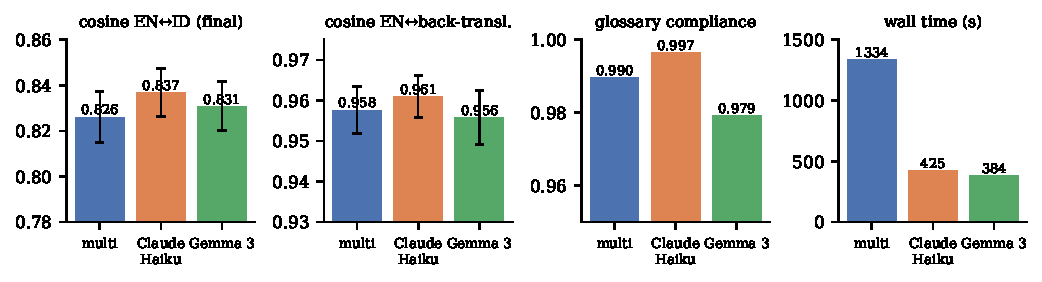
\includegraphics[width=0.95\textwidth]{fig2_configs.pdf}
  \caption{Eksperimen B: kualitas teks akhir (cosine dengan galat baku), kepatuhan glosarium dan waktu dinding dari ketiga konfigurasi.}
  \label{fig:configs}
\end{figure*}

\paragraph{Apa yang dilakukan penyunting}
Pada \textsc{multi} penyunting mengubah 38 dari 146 unit (26\%); rasio suntingan rata-rata di semua unit adalah 0.017, dan pada unit yang diubah 0.067 (maksimum 0.625). Seleksi QA mempertahankan teks yang ditinjau untuk 139 unit dan draf untuk 7 (Gambar~\ref{fig:review}a); kedua kandidat berada dekat diagonal, yaitu\ penyuntingan pasca jarang mengubah skor otomatis. Catatan perubahan menjelaskan koreksi terminologi dan tata bahasa: \emph{inferred} yang di-render sebagai ``diturunkan'' (derived) dikoreksi menjadi ``disimpulkan''; \emph{show} yang di-render sebagai ``dibuktikan'' (proven) menjadi ``ditunjukkan''; sebuah calque bertanda hubung ``sembilan-aturan'' menjadi ``dengan sembilan aturan''; dan satu kalimat bahasa Inggris lengkap yang model pembuat draf tinggalkan tanpa terjemahan pada paragraf pembuka diterjemahkan. Tidak satupun dari hal ini terlihat pada cosine rata-rata.

\begin{figure*}[t]
  \centering
  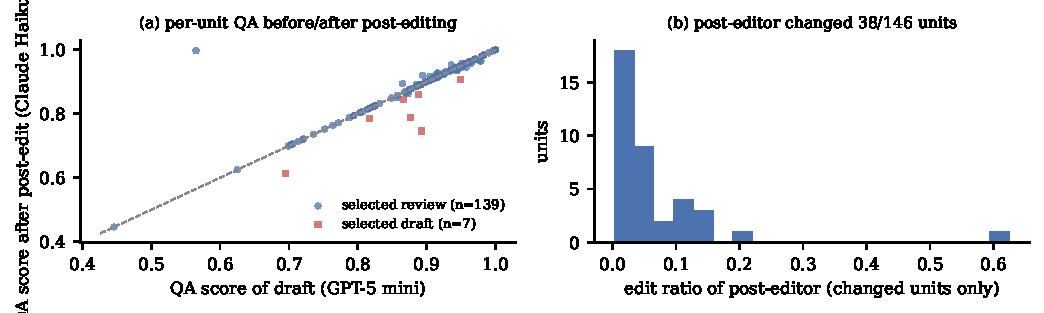
\includegraphics[width=0.95\textwidth]{fig3_review.pdf}
  \caption{\textsc{multi} pipeline: (a) skor QA per unit dari draf dan dari teks pasca-sunting dengan kandidat yang dipilih; (b) distribusi rasio suntingan oleh penyunting atas 38 unit yang diubah.}
  \label{fig:review}
\end{figure*}

\subsection{Eksperimen C: Siapa yang Menemukan Kesalahan Mana}
Tabel~\ref{tab:errors} mengklasifikasikan kesalahan yang kami temukan menurut lapisan yang menangkapnya. Tiga kelas tertangkap oleh validator dan tidak oleh apa pun selain itu. (i) \emph{Placeholder dipindahkan}: pada satu run pilot, penyunting, saat ``merapikan'' format angka, memindahkan placeholder untuk \verb|\%| ke depan angka (``hanya \ph{3}58'' untuk ``only 58\%''); pemeriksaan multiset lulus, sehingga aturan menempel pada angka ditambahkan dan sekarang menolak keluaran semacam itu. (ii) \emph{Terjemahan balik yang menggemakan}: pada 37 panggilan untuk unit pendek (33 kandidat hasil penyuntingan pasca dan 4 kandidat draf) model QA lokal mengembalikan teks bahasa Indonesia tanpa perubahan alih-alih bahasa Inggris; karena terjemahan balik kemudian sama dengan kandidat, cosine terjemahan balik runtuh (19 unit turun lebih dari 0.10) dan selektor keliru memilih draf untuk 25 unit yang dua kandidatnya identik. Aturan gema mengubah ini menjadi panggilan yang gagal untuk dicoba ulang, setelah itu seleksi menjadi 139/7. (iii) \emph{Placeholder yang hilang}: model lokal sebagai penerjemah tunggal kehilangan placeholder dalam dua paragraf meskipun sudah dicoba ulang; tanpa model cadangan (fallback) ini tetap dalam bahasa Inggris dan dilaporkan, yang merupakan perilaku yang benar. Kesalahan yang tertangkap oleh model bersifat semantik: sebuah kalimat yang tidak diterjemahkan, istilah teknis yang salah (\emph{confounder} menjadi ``perusak'' (destroyer) pada run lokal dan ``perancu'' atau ``konfonder'' di tempat lain; ``stokhastisitas'' salah eja), sebuah sel tabel ``Union'' yang dibiarkan dalam bahasa Inggris dan sebuah judul yang dipangkas menjadi ``Kritikus lintas'' pada satu run Claude Haiku---ketiga terakhir ditemukan melalui pembacaan manusia, yang tetap menjadi lapisan terakhir.

\begin{table}[t]
  \caption{Eksperimen C: kelas kesalahan dan lapisan yang menangkapnya (P = model penyuntingan pasca, Q = model QA, V = validator deterministik, H = pembacaan manusia).}
  \label{tab:errors}
  \centering
  \small
  \begin{tabular}{@{}p{4.1cm}cp{2.6cm}@{}}
    \toprule
    Kesalahan & Tertangkap oleh & Kejadian \\
    \midrule
    Placeholder dipindahkan sebelum angka & V & 1 unit (pilot) \\
    Model QA menggemakan inputnya & V & 37 panggilan \\
    Placeholder yang hilang (model lokal) & V & 2 unit \\
    Kalimat tidak diterjemahkan & P & 1 unit \\
    Istilah teknis salah & P, H & 4 istilah \\
    Ejaan salah (``stokhastisitas'') & H & 1 unit \\
    Sel atau judul dibiarkan/terpotong & H & 2 unit (Claude Haiku) \\
    \bottomrule
  \end{tabular}
\end{table}

\subsection{Jawaban terhadap Pertanyaan Penelitian}
\textbf{RQ1.} Tidak: SDK vendor dapat menyajikan model yang berbeda dari yang diminta tanpa menghasilkan kesalahan apa pun, dan satu-satunya label yang benar adalah model yang disebutkan dalam event penggunaan; agen merekamnya untuk setiap panggilan. \textbf{RQ2.} Pipeline tiga-model tidak meningkatkan kualitas rata-rata---sebuah model kuat tunggal menyamai atau melampauinya dalam sepertiga waktu---dan integritas struktur merupakan sifat dari validator daripada dari pipeline (kedua konfigurasi API-model mencapai 146/146); yang ditambahkan oleh pipeline adalah koreksi terhadap kesalahan semantik yang tidak ditunjukkan oleh metrik mana pun. \textbf{RQ3.} Kesalahan struktural dan protokol (placeholder, gema) hanya ditangkap oleh validator; kesalahan semantik ditangkap oleh model kedua atau oleh peninjau manusia.

\section{Diskusi}
\label{sec:discussion}

\paragraph{Rata-rata versus penangkapan kesalahan}
Ketiga konfigurasi secara statistik tidak dapat dibedakan pada metrik otomatis, dan model tunggal yang kuat adalah cara termurah untuk mencapai tingkat tersebut. Seandainya kami hanya mengevaluasi berdasarkan mean cosine, kami akan menyimpulkan bahwa pipeline multi-model adalah upaya yang sia-sia. Tinjauan per-unit mengatakan sebaliknya: integritas struktur berasal dari validator (kedua konfigurasi Copilot mencapai 146/146, model lokal 144/146), dan penyunting pada pipeline memperbaiki kesalahan semantik---sebuah kalimat yang tidak diterjemahkan, tiga istilah yang salah---yang tidak dicatat oleh metrik karena sebuah kalimat yang dibiarkan dalam bahasa Inggris masih memiliki embedding yang mirip dengan sumbernya. Hal ini sesuai dengan pengamatan bahwa manfaat panggilan LLM tambahan bergantung pada di mana kesalahan berada, bukan pada berapa banyak panggilan yang dilakukan~\cite{chen2024compound}: untuk sebuah dokumen di mana sebagian besar unit sudah diterjemahkan dengan baik, model kedua sebagian besar setuju (108 dari 146 unit tidak berubah) dan membenarkan biayanya pada beberapa unit yang diubahnya.

\paragraph{Validator adalah lapisan termurah dan satu-satunya yang melihat tiga kelas kesalahan}
Placeholder yang dipindahkan, terjemahan balik yang menggemakan, dan placeholder yang hilang tidak dapat dideteksi oleh model yang membaca teks yang lancar, dan model penilai itu sendiri merupakan sumber salah satunya. Pemeriksaan kesetaraan himpunan, ekspresi reguler untuk placeholder yang menempel pada angka, dan perbandingan string menangkap ketiganya dengan biaya yang sangat kecil. Ini adalah pelajaran yang sama yang memotivasi sistem pendamping~\cite{arya2026wizard}, di mana lapisan aturan simbolik memvalidasi keluaran LLM: sebuah LLM-sebagai-penilai~\cite{zheng2023judge} harus dinilai juga, dan penilai terakhir sebaiknya deterministik ketika sifatnya formal. Hal ini juga menyarankan desain untuk penggunaan produksi---\emph{review selektif}: jalankan satu model kuat dengan validator pada setiap unit, dan kirim ke model kedua hanya unit yang diberi tanda oleh validator atau heuristik murah (cosine rendah, kata fungsi bahasa sumber yang tersisa, istilah glosarium yang terlewat, placeholder yang berulang). Pada data kami, filter semacam itu akan mengarahkan sekitar sepersepuluh hingga seperempat unit, mendekati biaya model tunggal dengan kemampuan pipeline dalam menangkap kesalahan.

\paragraph{Model lokal untuk pemrosesan massal, model API untuk pass akhir}
Model lokal 27B adalah yang tercepat, tidak memiliki kuota, dan mencapai 97.9\% kepatuhan glosarium, tetapi ia menghapus placeholder pada dua paragraf dan menghasilkan satu-satunya istilah teknis yang jelas salah. Dalam pipeline yang dilayaninya, mode kegagalannya berbiaya rendah: terjemahan balik untuk QA (di mana sebuah gema terdeteksi secara deterministik) dan cadangan (fallback). Model mana yang mengisi peran mana harus mengikuti hak akses (entitlement) akun dan profil kesalahan tugas, oleh karena itu peran, bukan nama model, adalah unit konfigurasi.

\paragraph{Provenans}
Tanpa membaca event penggunaan (usage event), paper ini akan melaporkan pekerjaan Haiku sebagai milik Opus. Model yang diminta adalah nilai konfigurasi; model yang melayani adalah sebuah pengamatan, dan hanya pengamatan yang masuk dalam catatan ilmiah. Kami merekomendasikan agar agen riset (i) mencatat model yang melayani per panggilan, (ii) memberi label pada keluaran dengannya, (iii) memperingatkan jika terjadi substitusi model, dan (iv) memperlakukan kegagalan autentikasi sebagai kegagalan kesehatan alih-alih sebagai hasil kosong. Model cards~\cite{mitchell2019modelcards} menjelaskan model; agen tetap harus menentukan kartu mana yang berlaku.

\section{Keterbatasan}
\label{sec:limits}
Setiap konfigurasi dijalankan satu kali; keluaran LLM bervariasi antar run~\cite{arya2026wizard}, dan perbedaan yang kami laporkan antar konfigurasi (sekitar 0.01 pada cosine) berada dalam variabilitas tersebut. Semua metrik kualitas bersifat otomatis; cosine lintas bahasa dan cosine terjemahan balik adalah proksi yang diketahui gagal menangkap kesalahan terminologi dan kefasihan~\cite{freitag2021mqm,moon2020roundtrip}, yang tepat merupakan area di mana penyunting bertindak---evaluasi manusia oleh pakar domain dwibahasa diperlukan untuk mengkuantifikasi manfaat tersebut. Satu pasangan bahasa, satu tipe dokumen, dan satu glosarium dipelajari. Perbandingan tersebut mengaburkan pilihan model dengan peran penyuntingan pasca: validator aktif di semua konfigurasi, sehingga hasil struktural mengisolasi mereka, tetapi satu putaran penyuntingan pasca oleh model \emph{sama} dengan draf tidak diuji. Model QA juga berfungsi sebagai model cadangan (fallback), sehingga kelemahan sistematis Gemma 3 27B akan memengaruhi dua peran. Eksperimen A berkaitan dengan satu SDK vendor dan satu tingkat akun pada satu titik waktu; perilaku dapat berubah, dan penyedia lain mungkin menolak model yang tidak dikenal. Tinjauan dua-kritikus dan pengonversi DOCX adalah bagian dari agen yang dirilis tetapi tidak dievaluasi di sini.

\section{Kesimpulan}
\label{sec:conclusion}
Kami mendokumentasikan bahwa sebuah vendor SDK dapat senyap melayani model yang berbeda dari yang diminta dan mengubah event penggunaan yang mengungkapkannya menjadi mekanisme provenans bagi agen riset. Di sekitarnya kami membangun paper-agent, yang merutekan tugas penanganan paper ke model berdasarkan peran dan memvalidasi setiap keluaran model secara deterministik. Dalam perbandingan terkontrol pada 146 unit LaTeX, sebuah pipeline tiga-model tidak mengungguli satu model tunggal pada kualitas rata-rata atau pada integritas struktur---keduanya berasal dari validator---tetapi pipeline itu memperbaiki kesalahan semantik yang tidak terlihat oleh metrik; para validator menangkap tiga kelas kesalahan yang tidak terdeteksi oleh model mana pun, termasuk penilai. Penelitian lanjutan adalah evaluasi manusia terhadap koreksi penyunting, sebuah filter terpelajar untuk review selektif, dan memperluas provenans model yang melayani ke SDK lain. Sebagai pemeriksaan akhir, agen menerjemahkan paper ini ke Bahasa Indonesia dengan pipeline yang sama (131 unit, 4{,}200 kata; 131/131 unit secara struktural utuh; kepatuhan glosarium 95.7\%; cosine 0.88 langsung dan 0.96 terjemahan balik; model yang melayani GPT-5 mini, Claude Haiku 4.5 dan Gemma 3 27B); kedua versi dikompilasi dari bibliografi yang sama. Kode, metrik per-unit dan kedua versi bahasa dirilis di \url{https://github.com/devnolife/paper-agent}.


\bibliographystyle{IEEEtran}
\bibliography{references}

\end{document}
